\title{Aula 1 - Apresentação do curso}



\begin{frame}
    \titlepage
\end{frame}

\begin{frame}{Literatura}
    \centering
    \begin{columns}
        \begin{column}{0.5\linewidth}
            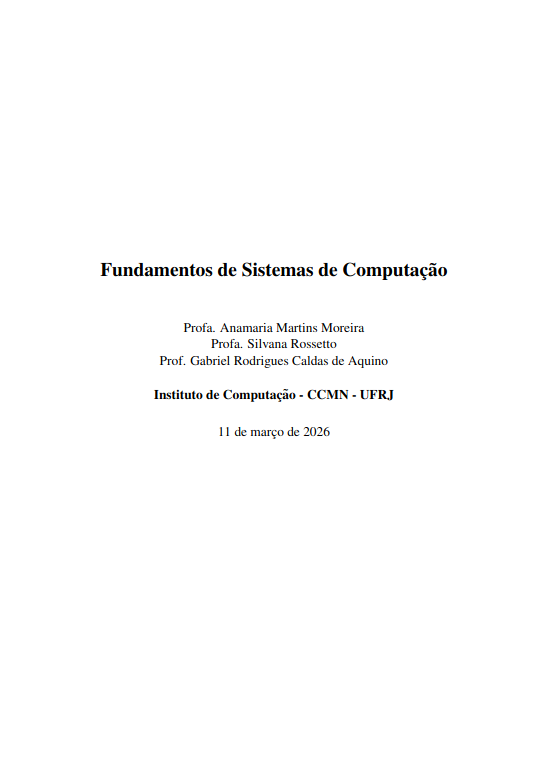
\includegraphics[width=0.8\linewidth]{Figuras/apostfund.png}
        \end{column}
        \begin{column}{0.5\linewidth}
            \begin{itemize}
                \item Apostila de fundamentos
                \item \href{URL}{Baixe a apostila}
            \end{itemize}
        \end{column}
    \end{columns}

\end{frame}

\begin{frame}{Literatura}
    \centering
    \begin{columns}
        \begin{column}{0.5\linewidth}
            \begin{itemize}
                \item Sistemas digitais: princípios e aplicações \\ Ronald J.
                      Tocci, Neal S. Widmer, Gregory L. Moss; \\ tradução
                      Jorge Ritter; revisão técnica Renato Giacomini. – 11. ed.
                      – São Paulo: Pearson Prentice Hall, 2011.
                      \\Título original: Digital systems: principles and applications
                      \\ISBN 978-85-430-0694-9
            \end{itemize}
        \end{column}
        \begin{column}{0.5\linewidth}
            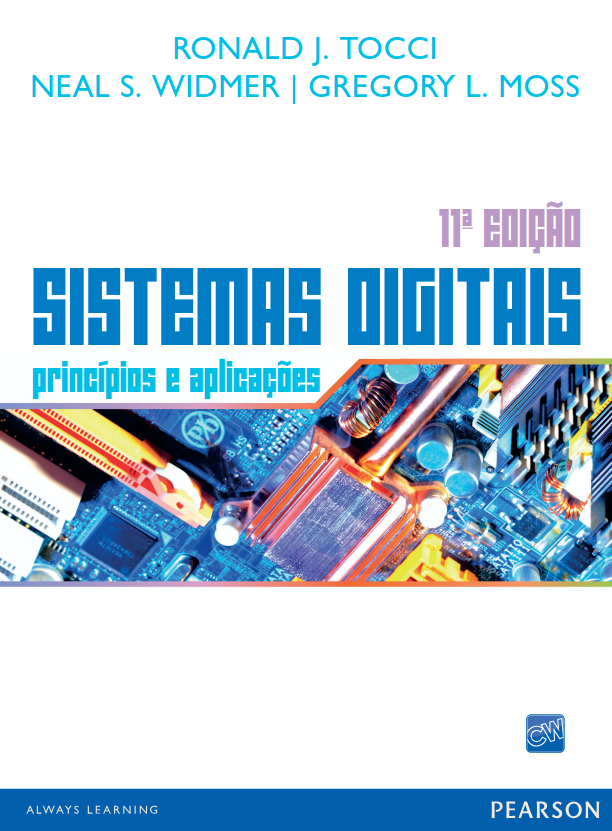
\includegraphics[width=0.8\linewidth]{Figuras/livro-sistdig.png}
        \end{column}
    \end{columns}

\end{frame}


\begin{frame}{Método de Avaliação}
    \textbf{Componentes da Nota}
    \begin{itemize}
        \item \textbf{Provas (P1, P2 e P3):}
              Média das provas (MP) $\rightarrow$ 80\% da nota

    \end{itemize}


    \textbf{Critério de Aprovação Direta}
    \begin{itemize}
        \item Média ponderada de das provas (P1, P2 e P3) $\geq 7$
              \hspace{1em} $\rightarrow$ Aprovado direto
        \item Se $3 <= \text{Média ponderada } <= 7$
              \hspace{1em} $\rightarrow$ Prova final (PF)
    \end{itemize}


    \textbf{Cálculo da Média Final}
    \[
        \text{Média final} = \frac{\text{Média anterior} + \text{PF}}{2}
    \]
    \begin{itemize}
        \item Se $\text{Média final} \geq 5$ $\Rightarrow$ Aprovado
        \item Caso contrário $\Rightarrow$ Reprovado
    \end{itemize}


\end{frame}


